\documentclass[conference]{IEEEtran}
\usepackage{cite}
\usepackage{amsmath,amssymb,amsfonts}
\usepackage{algorithmic}
\usepackage{graphicx}
\usepackage{textcomp}
\usepackage{xcolor}
\usepackage{hyperref}
\usepackage{float}
\usepackage{colortbl}
\usepackage{array}
\usepackage{amsmath}
\usepackage{multirow}
\usepackage{placeins}

\def\BibTeX{{\rm B\kern-.05em{\sc i\kern-.025em b}\kern-.08em
    T\kern-.1667em\lower.7ex\hbox{E}\kern-.125emX}}
\makeatletter % changes the catcode of @ to 11
\newcommand{\linebreakand}{%
  \end{@IEEEauthorhalign}
  \hfill\mbox{}\par
  \mbox{}\hfill\begin{@IEEEauthorhalign}
}

\definecolor{customcolor}{RGB}{64, 162, 227}
\colorlet{customtransparent}{customcolor!50}

\makeatother % changes the catcode of @ back to 12
\renewcommand{\arraystretch}{1.2}

\begin{document}
\title{A Comparative Analysis of Time Series Forecasting Models for Predicting Stock Prices in the Vietnamese Real Estate Sector}

\author{
\IEEEauthorblockN{Nhung Tran Thi Hong}
\IEEEauthorblockA{\textit{University of Information Technology} \\
Ho Chi Minh City, Viet Nam \\
\href{mailto:21522438@gm.uit.edu.vn}{21522438@gm.uit.edu.vn}}
\and
\IEEEauthorblockN{Quynh Do Mai Nhu}
\IEEEauthorblockA{\textit{University of Information Technology} \\
Ho Chi Minh City, Viet Nam \\
\href{mailto:21520429@gm.uit.edu.vn}{21520429@gm.uit.edu.vn}}
\and
\IEEEauthorblockN{Thuc Nguyen Huy}
\IEEEauthorblockA{\textit{University of Information Technology}\\
Ho Chi Minh City, Viet Nam \\
\href{mailto:21521505@gm.uit.edu.vn}{21521505@gm.uit.edu.vn}}
\and
\linebreakand
\IEEEauthorblockN{Thang Hoang Manh}
\IEEEauthorblockA{\textit{University of Information Technology} \\
Ho Chi Minh City, Viet Nam \\
\href{mailto:21521428@gm.uit.edu.vn}{21521428@gm.uit.edu.vn}}
\and
\IEEEauthorblockN{Dat Nguyen Duy}
\IEEEauthorblockA{\textit{University of Information Technology} \\
Ho Chi Minh City, Viet Nam \\
\href{mailto:21521936@gm.uit.edu.vn}{21521936@gm.uit.edu.vn}}
}

\maketitle
\pagestyle{plain}

\begin{abstract}
Vietnam's real estate market serves as a critical pillar of the nation's economy. Understanding stock price movements of leading companies within this sector is therefore crucial for informed investment decisions. This study applies several time series analysis techniques to explore forecasting models, including Linear Regression, ARIMA, RNN, GRU, LSTM, VARMA, Fuzzy time series, XGBoost, FEDformer, and DLinear. By training forecasting models on historical stock price data, this study compares their effectiveness in predicting the stock prices of Vietnamese real estate corporations. The evaluation will utilize three key metrics: Root Mean Squared Error (RMSE), Mean Absolute Error (MAE), and Mean Absolute Percentage Error (MAPE).
\end{abstract}

\begin{IEEEkeywords}
Stock prices prediction, Linear Regression, ARIMA, RNN, GRU, LSTM, VARMA, Fuzzy time series, XGBoost, FEDformer, DLinear.
\end{IEEEkeywords}

\section{Introduction}
Vietnam's real estate market has experienced phenomenal growth in recent years. Fueled by robust economic growth and favorable investment conditions, the sector has attracted substantial foreign investment. The stock market offers an alternative approach to participate in the real estate market's growth. Through shares of publicly traded real estate companies, investors can gain exposure to the sector without the complexities of direct property ownership. \par
Time series is a method which is used for the prediction of share prices. Time series analysis deals with analyzing a series of data gathered during time, which tries to forecast future by assuming that the previously observed patterns can be considered as the foundation to extract future behavior. \par
Stock market analysis is a challenging domain, characterized by a complex multivariate and time-evolving nature, with high volatility, and multiple correlations with exogenous factors. This study focuses on understanding and comparing the performance of several models for forecasting Vietnamese real estate stock prices using time series analysis techniques, including Linear Regression, ARIMA, RNN, GRU, LSTM, VARMA, Fuzzy time series, XGBoost, FEDformer and DLinear. \par
To provide a comprehensive comparison, this study will use historical stock price data starting from March 1st 2017 of three prominent Vietnamese real estate corporations: NVL (Novaland Group), KDH (Khang Dien House) and DXG (Dat Xanh Group).

\section{Related works}
Recently, there has been a significant surge in research focusing on forecasting stock prices through the application of diverse machine learning, deep learning and statistical models. \par
C.Ebenesh et al. \cite{b1} attempted to develop two models, Linear Regression and LSTM. Proposed framework has been tested for the prediction of three stocks and it has shown that LR model depicted promising performance compared to the LSTM model.\par
J. A. Rusman et al. \cite{b2} implemented Machine Learning and Deep Learning models such as RNN models (LSTM, Bi-LSTM, GRU, and Multi-LSTM) and ARIMA models. The results show that LSTM and ARIMA stood out within other models.\par
C. James et al. \cite{b3} investigated simultaneously the relations among stock returns, real activity, inflation, and money supply changes using a vector autoregressive moving average (VARMA) model.\par
K. Senthamarai Kannan et al. \cite{b4} compared Fuzzy time series and ARIMA model when used to predict fuel prices in India. It is concluded that fuzzy time series model gives better results than other time series model.\par
Y. Zhang et al. \cite{b5} applied XGBoost algorithm model to forecast stock prices based on the daily time series characteristics of stocks. The results demonstrate that the model is able to capture the high-frequency time series fluctuation trend of the stock and obtain more accurate prediction results about the stock price.\par
T. Zhou et al. \cite{b6} proposed the combination of Transformer with the seasonal-trend decomposition method. They also developed a frequency enhanced Transformer termed as Frequency Enhanced Decomposed Transformer (FEDformer).\par
L. Jialin et al. \cite{b7} proposed a hybrid model (HI-IVMD-DLinear) comprising the Hampel identifier (HI), the improved variational mode decomposition (IVMD) optimized by gray wolf optimization (GWO), and DLinear for wind speed forecasting (WSF). The experimental results reveal the model is suited to WSF and DLinear has great prediction performance.

\section{Materials}
\subsection{Datasets}
This study examines the historical stock prices of three leading real estate companies in Vietnam: Novaland Group (NVL), Khang Dien House (KDH), and Dat Xanh Group (DXG), taken from \href{https://www.investing.com/}{Investing.com}. The data will cover the period from March 1, 2017 to June 1, 2024. \par
Table \ref{tb_description} describes the columns in the chosen datasets.
\begin{table}[H]
\caption{Datasets description}
\label{tb_description}
    \begin{tabular}{|>{\centering\arraybackslash}p{0.15\linewidth}|>{\centering\arraybackslash}p{0.75\linewidth}|}
        \hline
            \rowcolor{customtransparent} \textbf{Column} & \textbf{Description} \\ \hline
        Date & The date of the data point\\ \hline
        Price & The closing price of the stocks on the given date\\ \hline
        Open & The opening price of the stocks on the given date\\ \hline
        High & The highest price reached by the stocks during the trading session on the given date\\ \hline
        Low & The lowest price reached by the stocks during the trading session on the given date\\ \hline
        Vol. & The trading volume for the day, denoted in million of shares traded\\ \hline
        Change \% & The percentage change in the closing price compared to the previous day's closing price\\\hline
    \end{tabular}
\end{table}
Since this study explores datasets containing historical closing prices, only descriptive statistical data relating to column \textit{Price} will be listed.

\subsection{Descriptive statistics}
\begin{table}[H]
  \centering
  \caption{NVL, KDH, DXG’s descriptive statistics}
\begin{tabular}{|>{\columncolor{customtransparent}}c|>{\centering\arraybackslash}p{0.2\linewidth}|>{\centering\arraybackslash}p{0.2\linewidth}|>{\centering\arraybackslash}p{0.2\linewidth}|}
    \hline
     \rowcolor{customtransparent} & \textbf{NVL} & \textbf{KDH} & \textbf{DXG} \\ \hline
     \textbf{Count} & 1800 & 1800 & 1800 \\ \hline
     \textbf{Mean} & 39806.3506 & 24523.0734 & 16803.1879\\ \hline
     \textbf{Median} & 32738.5 & 20300 & 15391.4\\ \hline
     \textbf{Mode} & 34491 & 12910.1 & 18950\\ \hline
     \textbf{Std} & 22351.3231 & 9700.0272 & 7150.8501\\ \hline
     \textbf{Min} & 10250 & 8944.8 & 6066.5\\ \hline
     \textbf{25\%} & 26584 & 17752 & 11735.825\\ \hline
     \textbf{50\%} & 32738.5 & 20300 & 15391.4\\ \hline
     \textbf{75\%} & 42752 & 31200 & 19965.9\\ \hline
     \textbf{Max} & 92366 & 51636 & 46750\\ \hline
     \textbf{Kurtosis} & -0.3526 & -0.3415 & 2.9124\\ \hline
     \textbf{Skewness} & 0.9943 & 0.7184 & 1.5023\\ \hline
\end{tabular}
\end{table}

\begin{figure}[H]
    \centering
    \begin{minipage}{0.23\textwidth}
    \centering
    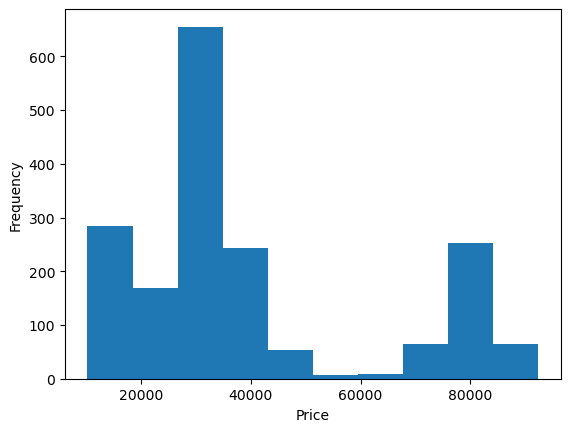
\includegraphics[width=1\textwidth]{figures/descriptive_stat/NVL_Histogram.png}
    \caption{NVL stock price's histogram}
    \label{fig_NVL_histogram}
    \end{minipage}
    \hfill
    \begin{minipage}{0.23\textwidth}
    \centering
    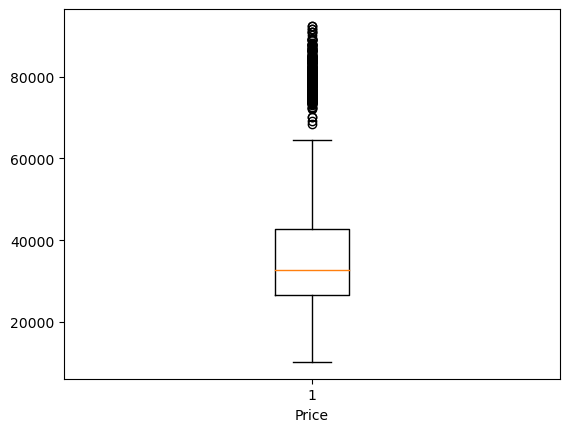
\includegraphics[width=1\textwidth]{figures/descriptive_stat/NVL_BoxPlot.png}
    \caption{NVL stock price's boxplot}
    \label{fig_NVL_bp}
    \end{minipage}
\end{figure}

\begin{figure}[H]
    \centering
    \begin{minipage}{0.23\textwidth}
    \centering
    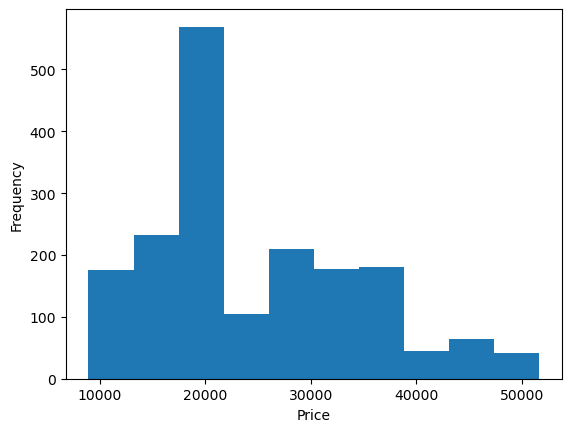
\includegraphics[width=1\textwidth]{figures/descriptive_stat/KDH_Histogram.png}
    \caption{KDH stock price's histogram}
    \label{fig_KDH_histogram}
    \end{minipage}
    \hfill
    \begin{minipage}{0.23\textwidth}
    \centering
    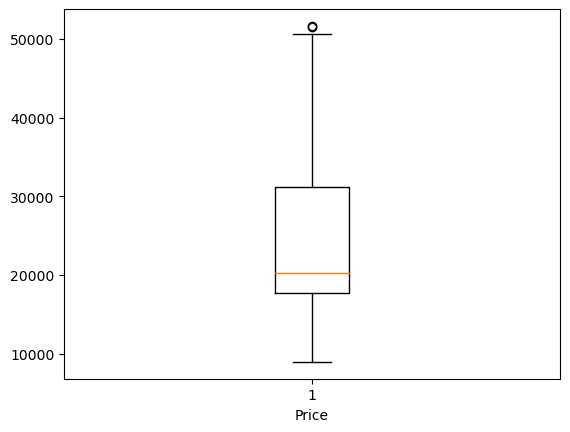
\includegraphics[width=1\textwidth]{figures/descriptive_stat/KDH_BoxPlot.png}
    \caption{KDH stock price's boxplot}
    \label{fig_KDH_bp}
    \end{minipage}
\end{figure}

\begin{figure}[H]
    \centering
    \begin{minipage}{0.23\textwidth}
    \centering
    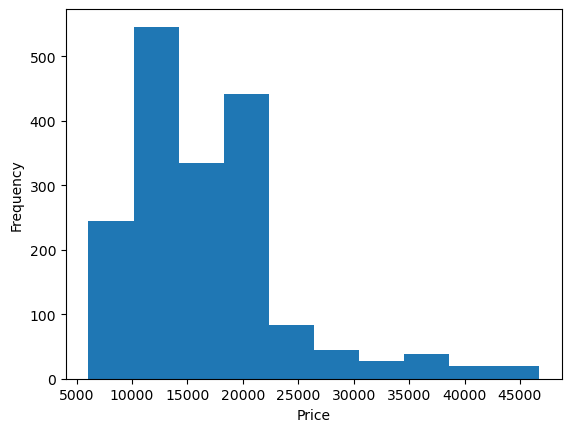
\includegraphics[width=1\textwidth]{figures/descriptive_stat/DXG_Histogram.png}
    \caption{DXG stock price's histogram}
    \label{fig_DXG_histogram}
    \end{minipage}
    \hfill
    \begin{minipage}{0.23\textwidth}
    \centering
    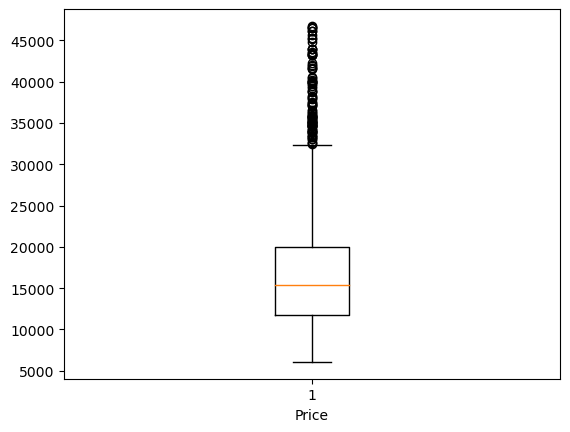
\includegraphics[width=1\textwidth]{figures/descriptive_stat/DXG_BoxPlot.png}
    \caption{DXG stock price's boxplot}
    \label{fig_DXG_bp}
    \end{minipage}
\end{figure}

\subsection{Data split ratio}
It was emphatically put that the size of datasets would be the determinant of split ratios that best fit the datasets so as to improve the model performance. Thus, determining the optimal allocation ratio between training and test sets is crucial. A commonly used ratio is 80:20, which means 80\% of the data is for training and 20\% for testing. Other ratios such as 70:30, 60:40, and even 50:50 are also used in practice. There does not seem to be clear guidance on what ratio is best or optimal for a given dataset \cite{b8}.\par
Therefore, in this study,  we decided to split the dataset into the ratios of  70:30, 80:20 and 90:10.  Ultimately, the choice of ratio will depend on the specific characteristics of the dataset and the goals of the analysis.

\subsection{Model evaluation metrics}
To assess the performance of the different forecasting models applied, we will utilize three key evaluation metrics: Root Mean Squared Error (RMSE), Mean Absolute Error (MAE), and Mean Absolute Percentage Error (MAPE).\par
\textbf{Root Mean Squared Error (RMSE)}: This metric calculates the square root of the average squared difference between the predicted and actual values.
\begin{equation}\label{eq_rmse}
RSME = \sqrt{\frac{1}{n}\sum_{i=1}^{n}(y_i - \hat{y}_i)^2}
\end{equation}\par
\textbf{Mean Absolute Error (MAE)}: This metric calculates the average of the absolute differences between predicted and actual values.
\begin{equation}\label{eq_mae}
MAE = \frac{1}{n}\sum_{i=1}^{n}|y_i - \hat{y}_i|
\end{equation}\par
\textbf{Mean Absolute Percentage Error (MAPE)}: This metric calculates the average error as a percentage relative to the actual values.
\begin{equation}\label{eq_mape}
MAPE = \frac{1}{n}\sum_{i=1}^{n}\left|\frac{y_i - \hat{y}_i}{y_i}\right| \times 100\%
\end{equation}\par
Where:\par
\begin{itemize}
    \item \(y_i\) is the actual value for the \textit{i}-th data point.
    \item \(\hat{y}_i\) is the predicted value for the \textit{i}-th data point.
    \item \textit{n} is the total number of data points.
\end{itemize}

\section{Methodology}
\subsection{Linear Regression}
Linear Regression is a statistical analysis method that characterizes linear relationships between a dependent variable and one or more independent variables. Eq. (\ref{eq_linear_regression}) describes the general form of a multivariable linear regression function.\par
\begin{equation}\label{eq_linear_regression}
Y = \beta_0 + \beta_1 X_1 + \beta_2 X_2 + \ldots + \beta_k X_k + \epsilon
\end{equation}\par
where:\par
\begin{itemize}
    \item \(Y\) is the dependent variable.\par
    \item \(X_1, X_2, ..., X_k\) are the independent variables.\par
    \item \(\beta_0\) is the intercept term.\par
    \item \(\beta_1, \beta_2, ..., \beta_k\) are the regression coefficients for the independent variables.\par
    \item \(\epsilon\) is the error term.
\end{itemize}

\subsection{ARIMA}
Autoregressive integrated moving average (ARIMA) is a popular statistical method used for time series forecasting. An ARIMA model includes the following components: Auto Regressive (AR), Integration (I) and Moving Average (MA).\par
An ARIMA model is defined by three parameters:\par
\begin{itemize}
    \item \(p\), which is the order of the Auto Regressive part (AR), indicates the number of lagged observations.
    \item \(d\), which is the degree of differencing or the number of times the data have had past values subtracted (to achieve stationarity).
    \item \(d\) is the order of the Moving Average part (MA), represents the number of lagged forecast errors.
\end{itemize}\par
The mathematical formula for an ARIMA(p, d, q) model can be represented as Eq. (\ref{eq_arima}).
\begin{equation}\label{eq_arima}
    \hat{y_t} = \mu + \phi_1y_{t-1} + ... + \phi_py_{t-p} - \theta_1e_{t-1} - ... - \theta_qe_{t-q}
\end{equation}\par
Where:
\begin{itemize}
    \item \(\mu\) is the constant term.
    \item \(\phi_1, ..., \phi_p\) are the coefficients of the AR part.
    \item \(y_{t-1}, ..., y_{t-p}\) are the previous observed values.
    \item \(\theta_1, ..., \theta_q\) are the coefficients of the MA part.
    \item \(e_{t-1}, ..., e_{t-q}\) are the residual terms.
\end{itemize}

\subsection{RNN}
Recurrent Neural Networks (RNN) is a type of Neural Network designed to work with sequential data like time series data and text data. RNN is different to other Neural Networks because it is capable of remembering information from previous steps with the help of hidden states.\par
RNN consists of an input layer, a hidden layer, and an output layer like other Neural Networks. But a hidden layer of RNN has neurons that take input not only from the input layer but also from the previous state due to an internal memory.\par
\begin{figure}[H]
    \centering
    \begin{minipage}{0.45\textwidth}
    \centering
    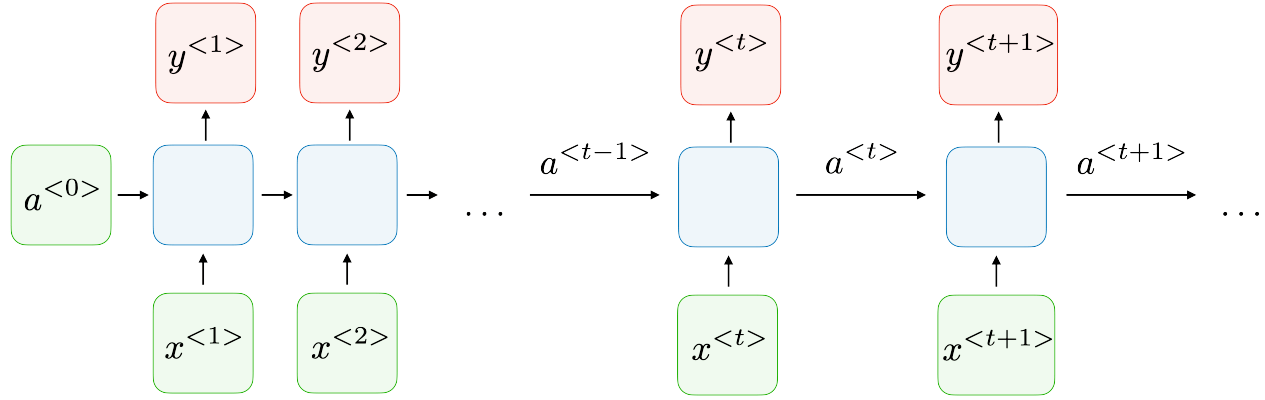
\includegraphics[width=1\textwidth]{figures/method/RNN_architecture.png}
    \caption{RNN architecture}
    \label{fig_RNN_architecture}
    \end{minipage}
\end{figure}\par
For each timestep \(t\), the activation \(a^{<t>}\) and the output \(y^{<t>}\) are expressed as Eq. (\ref{eq_rnn_at}) and Eq. (\ref{eq_rnn_yt}), respectively.
\begin{equation}\label{eq_rnn_at}
a^{<t>} = g_1(W_{aa}a^{<t-1>} + W_{ax}x^{<t>} + b_a)
\end{equation}
\begin{equation}\label{eq_rnn_yt}
y^{<t>} = g_2(W_{ya}a^{<t>} + b_y)
\end{equation}\par
Where:\par
\begin{itemize}
    \item \(W_{ax}, W_{aa}, W_{ya}, b_a, b_y\) are coefficients that are shared temporally.\par
    \item \(g_1, g_2\) are activation functions.
\end{itemize}
\begin{figure}[H]
    \centering
    \begin{minipage}{0.45\textwidth}
    \centering
    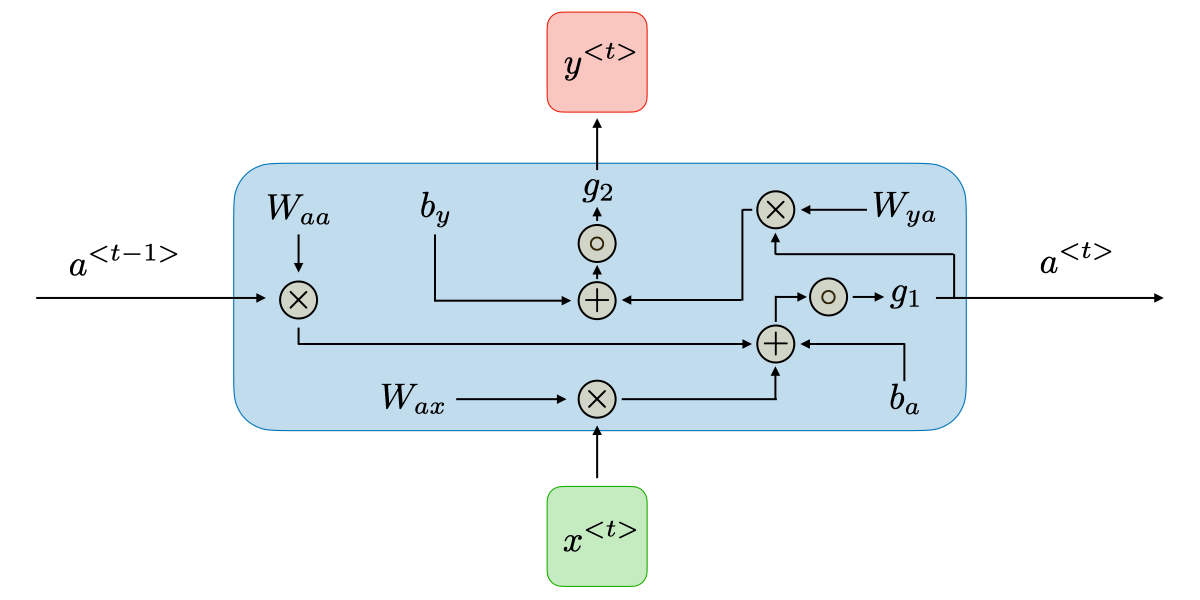
\includegraphics[width=1\textwidth]{figures/method/RNN_block.png}
    \caption{RNN block description}
    \label{fig_RNN_block}
    \end{minipage}
\end{figure}\par

\subsection{GRU}
A gated recurrent unit (GRU) was proposed by Cho et al. \cite{b9} to make each recurrent unit to adaptively capture dependencies of different time scales. Similarly to the LSTM unit, the GRU has gating units that modulate the flow of information inside the unit, however, without having a separate memory cells \cite{b10}. The structure of GRU is illustrated in Fig. \ref{fig_gru_structure}
\begin{figure}[H]
    \centering
    \begin{minipage}{0.45\textwidth}
    \centering
    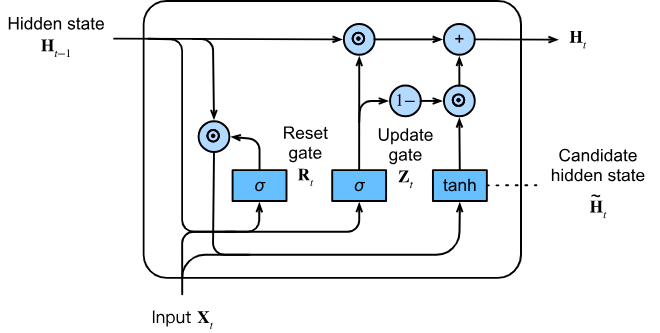
\includegraphics[width=0.9\textwidth]{figures/method/GRU_structure.png}
    \caption{The structure of GRU}
    \label{fig_gru_structure}
    \end{minipage}
\end{figure}\par
The activation \(h_t^i\) of the GRU at time \(t\) is a linear interpolation between the previous activation \(h_{t-1}^i\) and the candidate activation \(\Tilde{h_t^j}\), written as Eq. (\ref{eq_activation_gru}).
\begin{equation}\label{eq_activation_gru}
    h_t^j = (1-z_t^j)h_{t-1}^j + z_t^j\Tilde{h_t^j}
\end{equation}\par
where an update gate \(z_t^j\), written as Eq. (\ref{eq_update_gate_gru}) decides how much the unit updates its activation, or content.
\begin{equation}\label{eq_update_gate_gru}
    z_t^j = \sigma(W_zx_t + U_zh_{t-1})^j
\end{equation}\par
The candidate activation \(\Tilde{h_t^j}\) is computed as Eq. (\ref{eq_candidate_act_gru}).
\begin{equation}\label{eq_candidate_act_gru}
    \Tilde{h_t^j} = \tanh{(Wx_t + U(r_t \odot h_{t-1}}))^j
\end{equation}\par
where \(r_t\) is a set of reset gates and \(\odot\) is an element-wise multiplication.\par
The reset gate \(r_t^j\) is computed similarly to the update gate, described in Eq. (\ref{eq_reset_gate_gru}).
\begin{equation}\label{eq_reset_gate_gru}
    r_t^j = \sigma(W_rx_t + U_rh_{t-1})^j
\end{equation}

\subsection{LSTM}\label{method_LSTM}
The Long Short-Term Memory (LSTM) model is a recurrent neural network (RNN) which was designed as a solution to the dissatisfaction with RNN’s ability to capture long-term dependencies in sequential data.\par
The key feature of the LSTM model is the use of memory cells that can maintain information over long periods of time, allowing the network to learn and remember context from earlier in the sequence. LSTMs are composed of layers of memory blocks, each of which contains: cell state, forget gate, input gate, output gate. The structure of an LSTM model is illustrated in Fig. \ref{fig_LSTM_architecture}.
\begin{figure}[H]
    \centering
    \begin{minipage}{0.45\textwidth}
    \centering
    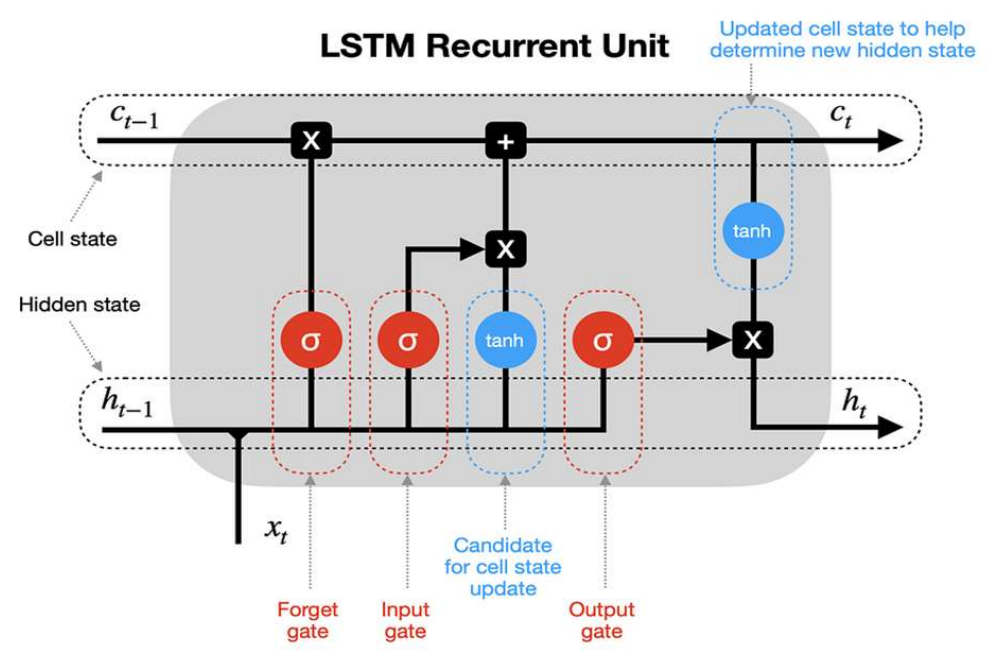
\includegraphics[width=1\textwidth]{figures/method/LSTM_Architecture.png}
    \caption{LSTM architecture}
    \label{fig_LSTM_architecture}
    \end{minipage}
\end{figure}\par
Mathematically, the nodes can be represented as:
\begin{align}
i_g &= \delta(W_{xi}X_{tt} + W_{hi}h_{tt-1} + W_{ci}C_{tt-1} + b_i)\label{eq_lstm_1} \\
f_g &= \delta(W_{xf}X_{tt} + W_{hf}h_{tt-1} + W_{cf}C_{tt-1} + b_f)\label{eq_lstm_2} \\
c_g &= f_tc_{t-1} + i_t\tanh(W_{xc}X_{tt} + W_{hc}h_{tt-1} + b_c)\label{eq_lstm_3} \\
o_g &= \delta(W_{xo}X_{tt} + W_{ho}h_{tt-1} + W_{co}c_t + b_o)\label{eq_lstm_4} \\
h_t &= o_g\tanh(c_t)\label{eq_lstm_5}
\end{align}\par
Eqs. (\ref{eq_lstm_1}) - (\ref{eq_lstm_5}) show the formation of various nodes, here \(i_g\), \(f_g\) and \(o_g\) being the input gate, forget gate and output gate respectively. The input of the LSTM is twofold process, where the current sample  \(X_{tt}\) is the previous hidden layer sample,  \(h_{tt-1}\) being the cell state and  \(c_{t-1}\) gives the internal source of each gate. While the activation function is given as \(\sigma\) and \(\tanh\).  \(W_{xf}\) is the weight matrix for signal \(a\) and  \(f\) \cite{b11}.

\subsection{VARMA}
The Vector Autoregression Moving-Average (VARMA) is a type of time series model used in econometrics and statistics to analyze and forecast the behavior of multiple time series variables.
\subsubsection{VAR model}\hfill\par
A Vector Autoregression or VAR model of order \(p\) (denoted as \(VAR(p)\)) is a system of equations where each variable in the system is regressed on its own lagged values and the lagged values of all other variables in the system.Eq. (\ref{eq_var}) describes the VAR model of \(k\) variables.
\begin{equation}\label{eq_var}
    Y_t = c + \phi_1Y_{t - 1} + \phi_2Y_{t - 2} + ... + \phi_pY_{t - p} + \epsilon_t
\end{equation}\par
Where:\par
\begin{itemize}
    \item \(Y_t\) is a \(k \times 1\) vector of variables at time \(t\).
    \item \(c\) is a \(k \times 1\) vector of constants.
    \item \(\phi_1, \phi_2, ..., \phi_k\) are \(k \times k\) coefficient matrices.
    \item \(\epsilon_t\) is a \(k \times 1\) vector of error terms, assumed to be multivariate normally distributed with mean zero and covariance matrix \(\sum\).
\end{itemize}
\subsubsection{MA model}\hfill\par
A moving-average model of order \(q\) (denoted as \(MA(q)\)) is a model that regresses the variable on past forecast errors. Eq. (\ref{eq_ma}) describes the MA model of \(k\) variables.
\begin{equation}\label{eq_ma}
    Y_t = \mu + \theta_1\epsilon_{t - 1} + \theta_2\epsilon_{t - 2} + ... + \theta_p\epsilon_{t - p} + a_t
\end{equation}\par
Where:\par
\begin{itemize}
    \item \(\mu\) is a \(k \times 1\) vector of means.
    \item \(\theta_1, \theta_2, ..., \theta_k\) are \(k \times k\) coefficient matrices.
    \item \(\epsilon_{t-1}, \epsilon_{t-2}, ..., \epsilon_{t-q}\) are the lagged forecast errors.
    \item \(a_t\) is a \(k \times 1\) vector of residuals, assumed to be multivariate normally distributed with mean zero and covariance matrix \(\sum\).
\end{itemize}
\subsubsection{Combining VAR and MA into VARMA model}\hfill\par
A \(VARMA(p, q)\) model is a combination of the \(VAR(p)\) and \(MA(q)\) models. Eq. (\ref{eq_varma}) expresses a VARMA model.
\begin{equation}\label{eq_varma}
    \begin{align}
        Y_t = c + \phi_1Y_{t - 1} + \phi_2Y_{t - 2} + ... + \phi_pY_{t - p} + \epsilon_t \\
    + \mu + \theta_1\epsilon_{t - 1} + \theta_2\epsilon_{t - 2} + ... + \theta_p\epsilon_{t - p} + a_t
    \end{align}
\end{equation}\par
Estimating the parameters (coefficient matrices \(\phi_1, \phi_2, \phi_p, \theta_1, \theta_2, \theta_q\)) of a VARMA model is typically done using maximum likelihood estimation or other methods like least squares.

\subsection{Fuzzy time series}
Fuzzy prediction for time series is an approach that applies the theory of fuzzy logic to make predictions about future data points in a time series. This approach is particularly useful when dealing with data that is uncertain, imprecise, or subject to vagueness.\par
Fuzzy time series models have been developed along two main directions: \textit{a)} Fuzzification of raw data to establish its association, followed by the application of a known model for future forecasting, and \textit{(b)} Direct construction of a forecasting model for the future. Compared to \textit{(b)}, the research direction \textit{(a)} has garnered more interest from statisticians.\par
\begin{figure}[H]
    \centering
    \begin{minipage}{0.45\textwidth}
    \centering
    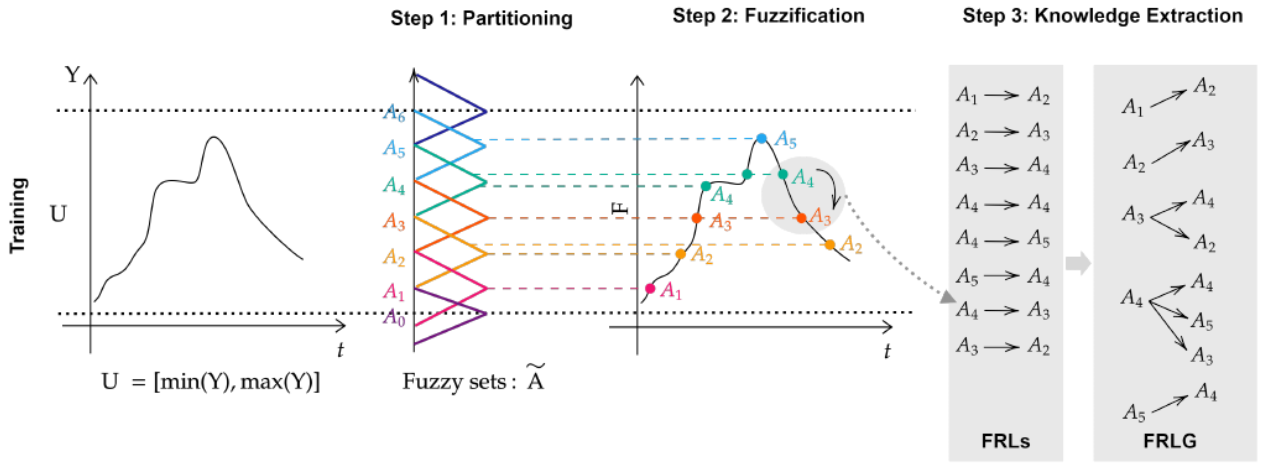
\includegraphics[width=1\textwidth]{figures/method/Fuzzy_Training.png}
    \caption{Training procedure of fuzzy time series model}
    \label{fig_fuzzy_training}
    \end{minipage}
\end{figure}
The training phase, illustrated in Fig. \ref{fig_fuzzy_training}, consists of stages 1 to 3 described below.\par
\textbf{Step 1 - Universe of Discourse partitioning}: First, define the universe of discourse. The universe of discourse U is defined as follows: take the maximum value \(f_{max}\) and the minimum value \(f_{min}\) of the time series, and \(U = [f_{max}, f_{min}]\). Sometimes, this range can be extended by adding an additional value for ease of computation. Then, divide the interval \(U\) into \(m\) equal sub-intervals \(u_1, u_2,.., u_m\).\par
\textbf{Step 2 - Fuzzification}:Determine the fuzzy sets \(A_i\) and fuzzify the values. Each \(A_i\) set is assigned a linguistic variable and determined on the identified segments \(u_1, u_2,.., u_m\).Then the fuzzy sets \(A\) can be represented as Eq. (\ref{eq_fuzzy_step2}):
\begin{equation}\label{eq_fuzzy_step2}
    A_i = \frac{\mu_{A_i}(u_1)}{u_1} + \frac{\mu_{A_i}(u_2)}{u_2} + ... + \frac{\mu_{A_i}(u_m)}{u_m}
\end{equation}\par
\textbf{Step 3 - Knowledge or Temporal Pattern Extraction}: Establish fuzzy relationships and group them. As defined above, for a fuzzy time series, fuzzy relationships can be identified at each time \(t\), thereby determining groups of fuzzy relationships.\par
For the forecasting procedure, it is illustrated in Fig. \ref{fig_fuzzy_forecasting}.\par
\begin{figure}[H]
    \centering
    \begin{minipage}{0.45\textwidth}
    \centering
    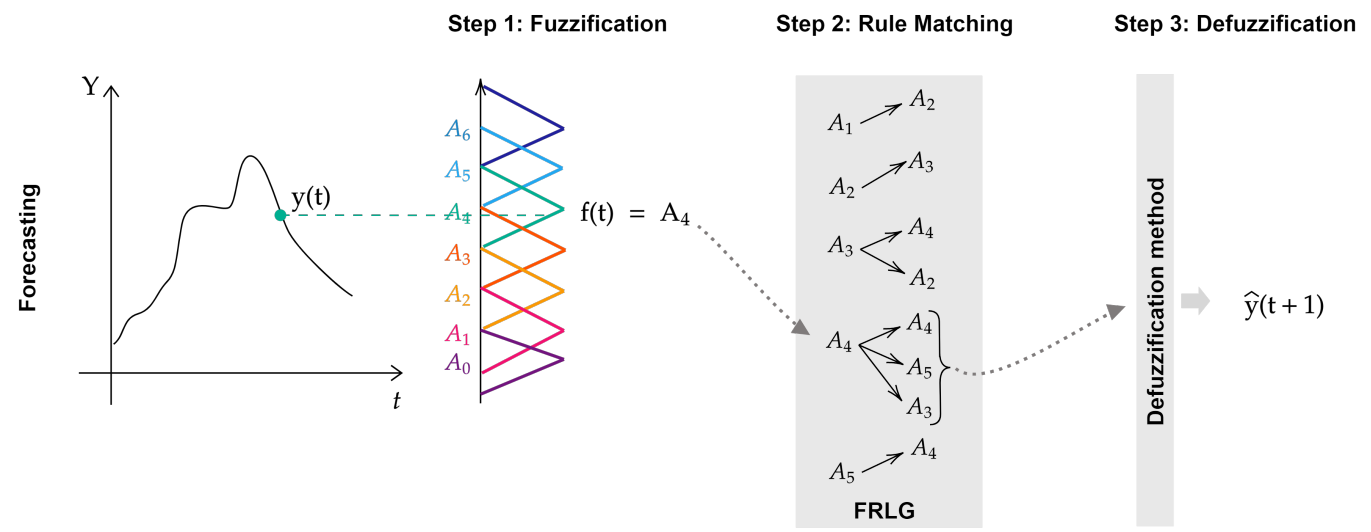
\includegraphics[width=1\textwidth]{figures/method/Fuzzy_Forecasting.png}
    \caption{Forecasting procedure of fuzzy time series model}
    \label{fig_fuzzy_forecasting}
    \end{minipage}
\end{figure}\par
\textbf{Step 1 - Fuzzification}: the fuzzification step is the same for both forecasting process and training procedure. It means that it translates the numeric sample \(y(t) \in Y\) into a fuzzy value \(f(t)\), where \(f(t) \in \Tilde{A}\).\par
\textbf{Step 2 - Rule Matching}: find the rules that contain the fuzzy set \(f(t)\) in its precedent. The activation of the rules are given by the membership values in \(f(t)\).\par
\textbf{Step 3 - Defuzzification}: the aim of this process is transforming the fuzzy value \(f(t+1)\) to a crisp value \(\hat{y}(t+1)\).In additions point forecasting methods, other types of defuzzification have been proposed for intervals and probabilistic distributions forecasting in the literature, see for instance.

\subsection{XGBoost}
Extreme Gradient Boosting (XGBoost) is a machine learning tool based on massively parallel Gradient Boosting (GB) as an enhanced version of the GB method, which is an algorithm based on residual optimization designed to achieve high efficiency, flexibility and portability.\par
XGBoost provides parallel boosting trees and establishes K regression trees, so that the predicted value of the tree group is close to the true value. It has strong generalization ability, and can quickly and accurately solve many scientific data problems. XGBoost is an improved algorithm of Gradient-boosted decision trees, and its core is the value of optimizing the objective function \cite{b12}.\par
\begin{figure}[H]
    \centering
    \begin{minipage}{0.45\textwidth}
    \centering
    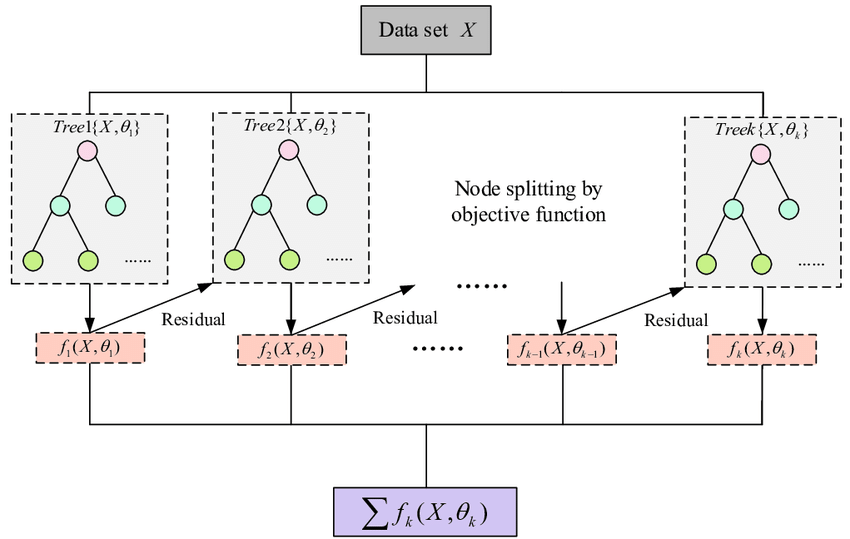
\includegraphics[width=1\textwidth]{figures/method/XGBoost_architecture.png}
    \caption{XGBoost architecture}
    \label{fig_XGBoost_architecture}
    \end{minipage}
\end{figure}
The objective function of XGBoost is typically formulated as a sum of a differentiable loss function \(l(y_i,\hat{y_i})\) and a regularization term \(\Omega(f)\) to prevent overfitting. The goal is to minimize this objective function.The objective function can be written as Eq. (\ref{eq_XGBoost}).
\begin{equation}\label{eq_XGBoost}
    Obj = \sum_{i=1}^{n} l(y_i, \hat{y}_i) + \sum_{k=1}^{K} \Omega(f_k)
\end{equation}\par
Where:\par
\begin{itemize}
    \item \(l(y_i,\hat{y_i})\) is the training error of sample \(x_i\).\par
    \item \(\Omega(f_k)\) is the regular term of the first tree.\par
    \item \(K\) is the total number of trees.\par
    \item \(f_k\) represents the \(k\) first trees.\par
    \item \(\hat{y_i}\) is the prediction result of sample \(x_i\).
\end{itemize}

\subsection{FEDFormer}
The FEDformer, also known as \textit{Frequency Enhanced Decomposed Transformer}, is a method for short-term and long-term time series prediction. It combines the Transformer model with a seasonal decomposition approach to address the high computational and memory requirements of Transformers for long time series.\par
\begin{figure}[H]
    \centering
    \begin{minipage}{0.45\textwidth}
    \centering
    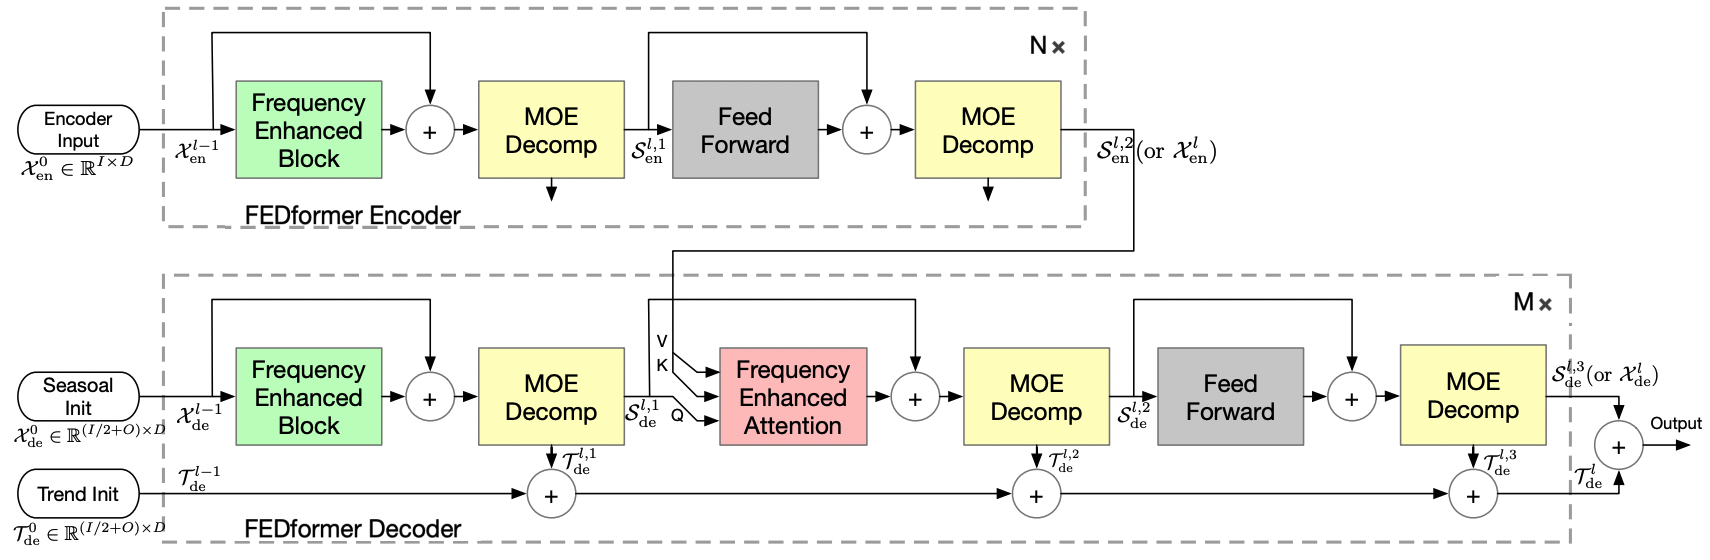
\includegraphics[width=1\textwidth]{figures/method/FEDFormer_structure.png}
    \caption{Overall structure of FEDFormer}
    \label{fig_fedformer}
    \end{minipage}
\end{figure}\par
\textbf{Structure} \textit{(illustrated in Fig. \ref{fig_fedformer})}: FEDFormer comprises of \(N\) encoders and \(M\) decoders. It integrates Frequency Enhanced Blocks (FEB) and Frequency Enhanced Attention (FEA) for representation learning in the frequency domain. These blocks come in two versions: FEB/FEA with Fourier basis (-f) and FEB/FEA with Wavelet basis (-w). The Mixture Of Expert Decomposition Blocks (MOEDecomp) are used to extract seasonal-trend patterns from the input data.\par
\textbf{Mixture of Experts for Seasonal-Trend Decomposition}: 
It contains a set of average filters with different sizes to extract multiple trend components from the input signal and a set of data-dependent weights for combining them as the final trend \cite{b6}. Its formula can be written as Eq. (\ref{eq_fed_trend}).
\begin{equation}\label{eq_fed_trend}
    X_{trend} = Softmax(L(x)) \times (F(x))
\end{equation}
Where:\par
\begin{itemize}
    \item \(F(\cdot)\) is a set of average pooling filters.
    \item \(Softmax(L(x))\) is the weights for mixing these extracted trends.
\end{itemize}

\subsection{DLinear}
DLinear is a novel high-precision time-series forecasting model proposed by A. Zeng et al. \cite{b13} in 2022. Despite its simple structure (illustrated in Fig. \ref{fig_dlinear_structure}), consisting solely of a decomposition scheme and two linear networks, its predictive accuracy exceeds that of the transformer model. It first decomposes a raw data input into a trend component \(X_t\) by a moving average kernel and a remainder component \(X_s = X - X_t\). Subsequently, two single-layer linear networks are utilized to forecast each of these decomposed components. The output results of the two single-layer linear networks are combined to yield the final predicted outcome \(\hat{X}\).
\begin{figure}[H]
    \centering
    \begin{minipage}{0.45\textwidth}
    \centering
    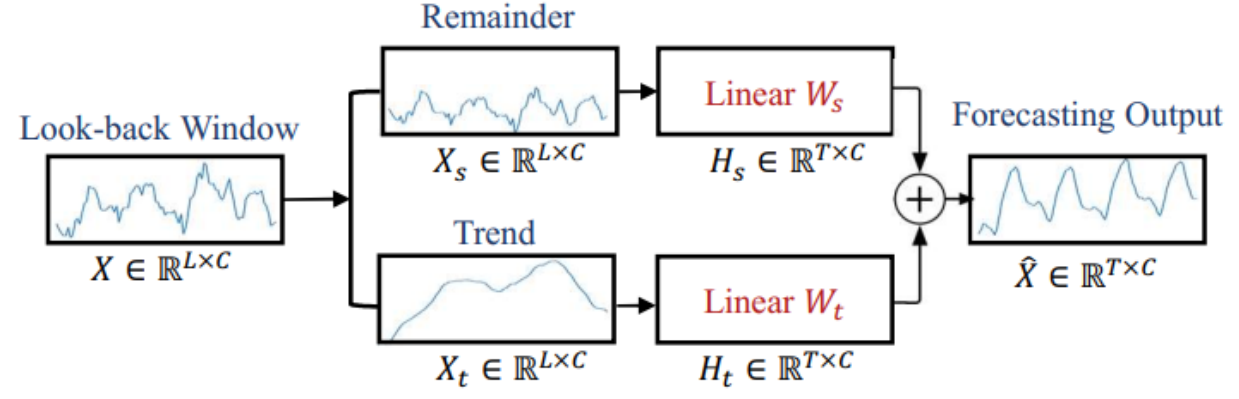
\includegraphics[width=1\textwidth]{figures/method/DLinear_structure.png}
    \caption{The whole structure of DLinear}
    \label{fig_dlinear_structure}
    \end{minipage}
\end{figure}\par
The whole process is \(\hat{X} = H_s + H_t\), where \(H_s = W_sX_s\) and \(H_t = W_tX_t\) are the decomposed trend and remainder figures. \(W_t \in R^{T \times L}\) and \(W_s \in R^{T \times L}\) are two linear layers, as illustrated in Fig. \ref{fig_dlinear_layer}.
\begin{figure}[H]
    \centering
    \begin{minipage}{0.45\textwidth}
    \centering
    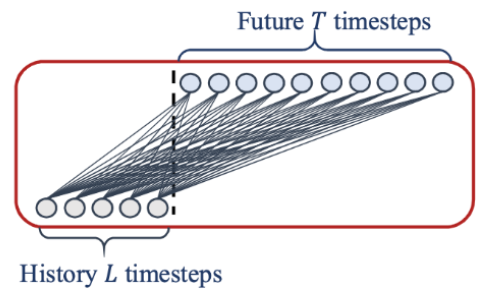
\includegraphics[width=0.8\textwidth]{figures/method/DLinear_Layer.png}
    \caption{One linear layer}
    \label{fig_dlinear_layer}
    \end{minipage}
\end{figure}\par

\section{Results}
The performance evaluation results of the time series forecasting methods on the testing set are shown in Table \ref{tb_evaluation}.
\FloatBarrier
\begin{table*}
    \centering
    \caption{Models evaluation for 3 datasets}
    \label{tb_evaluation}
    \begin{tabular}{|c|c|c|c|c|c|c|c|c|c|c|}
        \hline
        \multirow{2}{*}{\textbf{Model}} & \multirow{2}{*}{\textbf{Ratio}} & \multicolumn{3}{c|}{\textbf{NVL dataset}} & \multicolumn{3}{c|}{\textbf{KDH dataset}} & \multicolumn{3}{c|}{\textbf{DXG dataset}} \\ \cline{3-11}
        & & \textbf{RMSE} & \textbf{MAE} & \textbf{MAPE} & \textbf{RMSE} & \textbf{MAE} & \textbf{MAPE} & \textbf{RMSE} & \textbf{MAE} & \textbf{MAPE}\\ \hline
        \multirow{3}{*}{\textbf{Linear Regression}} 
            & 7:3 & 4847.4501 & 3675.0894 & 22.3727 & 21874.2175 & 21109.3975 & 71.5898 & 4847.4501 & 3675.0894 & 22.3727 \\ 
            & 8:2 & 4592.2668 & 3998.0721 & 32.1805 & 16224.0629 & 15716.7225 & 56.0464 & 4592.2668 & 3998.0722 & 32.1805 \\ 
            & 9:1 & 4847.4501 & 3675.0894 & 22.3727 & 11367.7932 & 11225.9241 & 40.8468 & 4928.9329 & 4663.3654 & 52.4450 \\ \hline
        \multirow{3}{*}{\textbf{ARIMA}} 
            & 7:3 & 100 & 100 & 100 & 100 & 100 & 100 & 100 & 100 & 100 \\
            & 8:2 & 100 & 100 & 100 & 100 & 100 & 100 & 100 & 100 & 100 \\
            & 9:1 & 100 & 100 & 100 & 100 & 100 & 100 & 100 & 100 & 100 \\ \hline
        \multirow{3}{*}{\textbf{RNN}} 
            & 7:3 & 1073.7004 & 605.8783 & 0.0263 & 675.1599 & 490.1798 & 0.0176 & 581.1192 & 419.8946 & 0.0267 \\
            & 8:2 & 537.8477 & 405.7168 & 0.0255 & 697.0829 & 558.3730 & 0.0182 & 603.8096 & 488.9243 & 0.0289 \\
            & 9:1 & 408.8307 & 313.1778 & 0.0193 & 580.0368 & 436.1019 & 0.0129 & 400.8059 & 284.3009 & 0.0156 \\ \hline
        \multirow{3}{*}{\textbf{GRU}} 
            & 7:3 & 100 & 100 & 100 & 100 & 100 & 100 & 100 & 100 & 100 \\
            & 8:2 & 100 & 100 & 100 & 100 & 100 & 100 & 100 & 100 & 100 \\
            & 9:1 & 100 & 100 & 100 & 100 & 100 & 100 & 100 & 100 & 100 \\ \hline
        \multirow{3}{*}{\textbf{LSTM}} 
            & 7:3 & 3057.0687 & 2581.9272 & 0.1450 & 2474.9107 & 2295.8782 & 0.0779 & 741.6859 & 487.7340 & 0.0310 \\
            & 8:2 & 1116.5333 & 992.8229 & 0.0658 & 1066.1759 & 916.1078 & 0.0294 & 513.0371 & 360.6441 & 0.0213 \\
            & 9:1 & 440.8700 & 325.3412 & 0.0200 & 607.9493 & 409.0105 & 0.0120 & 700.9022 & 636.4490 & 0.0345 \\ \hline
        \multirow{3}{*}{\textbf{VARMA}} 
            & 7:3 & 63786.8499 & 52600.8267 & 329.9603 & 23240.6669 & 21213.6416 & 71.2025 & 4414.2572 & 3848.7426 & 31.4104 \\
            & 8:2 & 63482.7402 & 61596.5217 & 400.3996 & 4933.7900 & 4282.7469 & 13.8019 & 6600.0675 & 6043.7100 & 57.7823 \\
            & 9:1 & 5448.1930 & 4903.2711 & 28.1549 & 2721.9087 & 2155.7150 & 6.4256 & 2743.1989 & 2240.5066 & 27.0063 \\ \hline
        \multirow{3}{*}{\textbf{Fuzzy time series}} 
            & 7:3 & 28502.4882 & 23052.7131 & 0.4523 & 4791.2323 & 3355.8568 & 0.1007 & 4179.7508 & 3301.3608 & 0.1677 \\
            & 8:2 & 34783.6060 & 33187.2260 & 0.6552 & 5064.1243 & 3625.1106 & 0.1091 & 4455.8584 & 3911.2167 & 0.2016 \\
            & 9:1 & 10591.0069 & 6387.4151 & 0.2232 & 1468.6545 & 1290.9884 &  0.0404 & 2717.6705 & 2190.0614 & 0.1097 \\ \hline
        \multirow{3}{*}{\textbf{XGBoost}} 
            & 7:3 & 14976.3418 & 11744.9988 & 0.7441 & 2971.3440 & 1333.3926 & 0.0941 & 2416.2441 & 1789.4221 & 0.0653 \\
            & 8:2 & 10325.4461 & 10089.4680 & 0.6651 & 506.0889 & 359.1250 & 0.0215 & 672.2229 & 475.3558 & 0.0156 \\
            & 9:1 & 561.3287 & 443.7371 & 0.0271 & 434.9773 & 295.8660 & 0.0164 & 601.8973 & 437.9176 & 0.0130 \\ \hline
        \multirow{3}{*}{\textbf{FEDFormer}} 
            & 7:3 & 59606.9147 & 51250.7585 & 3.2512 & 40518.5709 & 37338.4497 & 1.2735 & 11021.3645 & 9330.5654 & 0.5742 \\
            & 8:2 & 18558.0938 & 17874.4459 & 1.1975 &  13774.1822 & 11945.1227 & 0.3853 & 3493.1056 & 2646.0691 &  0.1591 \\
            & 9:1 & 4798.4457 & 4529.9021 & 0.2904 & 2970.2837 & 2601.1792 & 0.0829 & 0.2271.1483 & 1833.9879 & 0.1063 \\ \hline
        \multirow{3}{*}{\textbf{DLinear}} 
            & 7:3 & 84573.8402 & 72164.2981 & 455.2693 & 108031.5544 & 91226.9143 & 303.2510 & 22437.8018 & 21506.2863 & 140.1282 \\
            & 8:2 & 4114.5684 & 3648.5189 & 23.7230 & 26634.0106 & 22393.2118 & 71.0791 & 7010.9711 & 5901.5990 & 33.5445 \\
            & 9:1 & 7272.1234 & 6978.8770 & 44.3861 & 18331.7568 & 16315.0754 & 48.9144 & 2706.9245 & 2328.9474 & 13.3720 \\ \hline
    \end{tabular}
\end{table*}
\FloatBarrier
Lorem Ipsum is simply dummy text of the printing and typesetting industry. Lorem Ipsum has been the industry's standard dummy text ever since the 1500s, when an unknown printer took a galley of type and scrambled it to make a type specimen book. It has survived not only five centuries, but also the leap into electronic typesetting, remaining essentially unchanged. It was popularised in the 1960s with the release of Letraset sheets containing Lorem Ipsum passages, and more recently with desktop publishing software like Aldus PageMaker including versions of Lorem Ipsum.
\section{Predictions}

\section{Conclusion}
\subsection{Summary}
Based on the results of our experiments, 

\subsection{Future considerations}
After experimenting, we find out that this research has certain limitations. It has not yet implemented additional preprocessing steps such as removing influential outliers that could affect prediction results. Moreover, due to constraints on time and the multitude of algorithms, the models and methods have not been optimally tuned, and the study lacks experimentation with different time intervals in the past to improve forecasting accuracy.\par

\section*{Acknowledgment}
We would like to express our deepest gratitude to \textbf{\textit{Assoc. Prof. Nguyen Dinh Thuan}} for providing the essential knowledge and expertise that formed the foundation of this project. His profound understanding of the subject matter and his ability to convey complex concepts clearly and effectively have been invaluable. His guidance has significantly enhanced the depth and quality of this research.\par
We are also sincerely thankful to \textit{\textbf{TA. Nguyen Minh Nhut}} for his thoughtful advice and continuous support. His constructive feedback, practical suggestions, and encouragement have been crucial in navigating the challenges encountered during this project. His assistance has played a significant role in ensuring the successful completion of this work.\par
Together, their contributions have been instrumental in the development and completion of this project, and we are truly grateful for their support and mentorship.

\begin{thebibliography}{00}
\bibitem{b1} C. Ebenesh and K. Anitha, "A Novel Approach to Minimize the Mean Square Error in Predicting Stock Price Index using Linear Regression in Comparison with LSTM Model," in \textit{2022 International Conference on Sustainable Computing and Data Communication Systems (ICSCDS)}, Erode, India, 2022, pp. 1365-1370. doi: 10.1109/ICSCDS53736.2022.9760764.
\bibitem{b2} J. A. Rusman, K. Chunady, S. T. Makmud, K. E. Setiawan, and M. F. Hasani, "Crude Oil Price Forecasting: A Comparative Analysis of ARIMA, GRU, and LSTM Models," in \textit{2023 IEEE 9th International Conference on Computing, Engineering and Design (ICCED)}, Kuala Lumpur, Malaysia, 2023, pp. 1-6. doi: 10.1109/ICCED60214.2023.10425576.
\bibitem{b3} C. James, S. Koreisha, and M. Partch, "A VARMA Analysis of the Causal Relations Among Stock Returns, Real Output, and Nominal Interest Rates," \textit{The Journal of Finance}, vol. 40, pp. 1375-1384, 2019. doi: 10.1111/j.1540-6261.1985.tb02389.x.
\bibitem{b4} K. Senthamarai Kannan, M. SulaigaBeevi, and S. Syed Ali Fathima, "A Comparison of Fuzzy Time Series and ARIMA Model," \textit{International Journal of Scientific \& Technology Research}, 2019, vol. 8, no. 8, pp. 1872-1876.
\bibitem{b5} Y. Zhang, "Stock Price Prediction Method Based on XGboost Algorithm," in \textit{Proceedings of the 2022 International Conference on Bigdata Blockchain and Economy Management (ICBBEM 2022)}, 2022, pp. 595-603. doi: 10.2991/978-94-6463-030-5\_60.
\bibitem{b6} T. Zhou, Z. Ma, Q. Wen, X. Wang, L. Sun, R. Jin, and R. "FEDformer: Frequency Enhanced Decomposed Transformer for Long-term Series Forecasting," in \textit{Proceedings of the 39th International Conference on Machine Learning}, 2022, PMLR 162:27268-27286.
\bibitem{b7}L. Jialin, C. Gong, S. Chen, and N. Zhou. 2023. "Multi-Step-Ahead Wind Speed Forecast Method Based on Outlier Correction, Optimized Decomposition, and DLinear Model", \textit{Mathematics 11}, no. 12: 2746. doi: 10.3390/math11122746.
\bibitem{b8}V. R. Joseph, "\textit{Optimal ratio for data splitting}", \textit{Statistical Analysis and Data Mining: The ASA Data Science Journal}. 15 (2022), pp. 531–538. https://doi.org/10.1002/sam.11583.
\bibitem{b9}K. Cho, B. van Merrienboer, D. Bahdanau, and Y. Bengio. "On the properties of neural machine translation: Encoder-decoder approaches", 2014. \textit{arXiv preprint arXiv:1409.1259}.
\bibitem{b10}J. Chung, C. Gulcehre, K. Cho, and Y. Bengio. "Empirical Evaluation of Gated Recurrent Neural Networks on Sequence Modeling", 2014. \textit{arXiv preprint arXiv:1412.3555}.
\bibitem{b11}. "Gradient Boosting and LSTM Based Hybrid Ensemble Learning for Two Step Prediction of Stock Market". \textit{Journal of Advances in Information Technology}, 2023, vol. 14, no. 6. doi: 10.12720/jait.14.6.1254-1260.
\bibitem{b12} T. Liwei, F. Li, S. Yu, and G. Yuankai. "Forecast of LSTM-XGBoost in Stock Price Based on Bayesian Optimization," \textit{Intelligent Automation \& Soft Computing}, 2021, vol. 29, no. 3, pp. 855-868. doi: /10.32604/iasc.2021.016805.
\bibitem{b13}A. Zeng, M. Chen, L. Zhang, and Q. Xu. "Are Transformers Effective for Time Series Forecasting?", 2022. \textit{arXiv preprint arXiv:2205.13504}.
\end{thebibliography}
\vspace{12pt}

\end{document}
